\section{\textbf{Simulation}}\label{sec:3}

\begin{figure*}
\centering
	\begin{subfigure}{.45\textwidth}
    \centering
    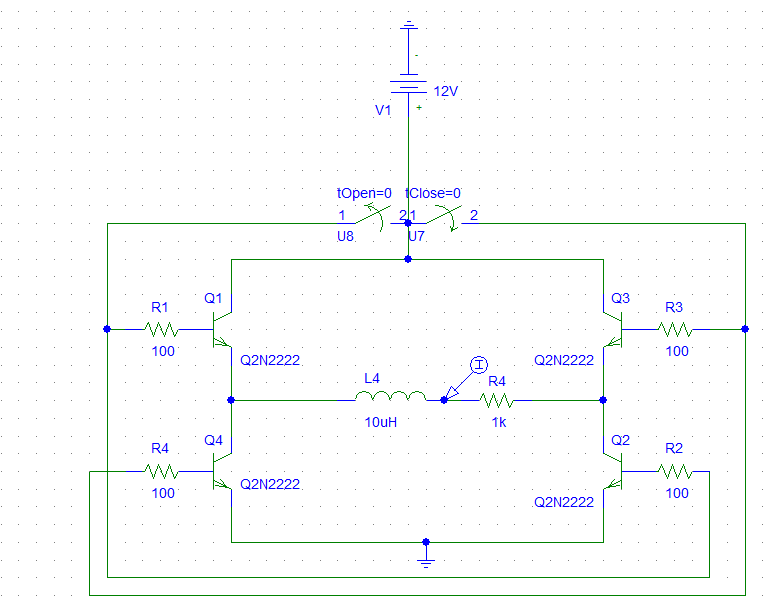
\includegraphics[width=\linewidth]{img/schem_pspice.png}
    \caption{Schematic on PSpice program.}\label{fig:schem_pspice}%
    \end{subfigure}    
    \begin{subfigure}{.45\textwidth}
    ~
    \centering
    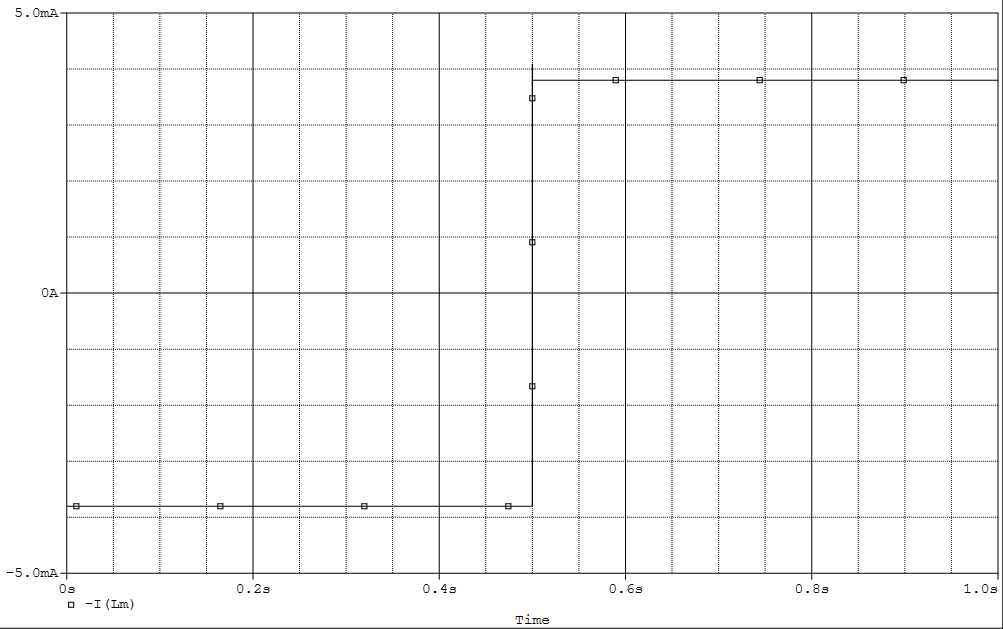
\includegraphics[width=\linewidth, height=6.4cm]{img/plot.png}
    \caption{Current x Time} \label{fig:plot_ponteh}
	\end{subfigure}
	\caption{Simulation analysis.}
	
\end{figure*}

    The circuit design was simulated using PSpice software distributed by OrCAD. The circuit shown in Figure~\ref{fig:schem} was reproduced in PSpice (see Figure \ref{fig:schem_pspice}). The software does not support the transistor model used in the actual implementation, the TIP31C, instead the Q2N2222 was used to replace it given they are very similar, only the maximum supported values for voltages change. The value of all transistors base resistances was set to $100\:\Omega$. The DC motor simplified equivalent circuit is an inductor and a resistor~\cite{CHAPMAN}. The U8 and U7 times were set to $500\; ms$.
\todo{TALK ABOUT THE MOTOR ITSELF}
	Finally a transient analysis over the circuit was made and the current flowing through the motor is plotted in Figure~\ref{fig:plot_ponteh}. The simulated circuit behavior is exactly the expected, when Q1 and Q2 are activated the current flows in the positive direction, in opposition to Q3 and Q4 active which results in a negative current flow.
	

